\documentclass[11pt]{article}
\usepackage[margin=0.7in]{geometry}\usepackage{graphicx}\usepackage[T1]{fontenc}\usepackage{hyperref}
\begin{document}\section*{Q0 image audit and Q1 transport failure}
T-1467, 3 November 2026, 19:45 UTC. Owner \texttt{3f18b4ff-4e50-4f17-8bd8-924fcca3958d}.

\textbf{Recorded outcome.} Q0 passed its image audit. Q1 emitted a held-gate observation with PID 1, UID/GID 1000, and pids.max/pids.current both 1. Its nonce and cgroup device/inode matched the host ancestry record. Release transport then failed: Docker copy exited 1 because the container root filesystem is read-only. Q1 did not pass; no automatic retry occurred.

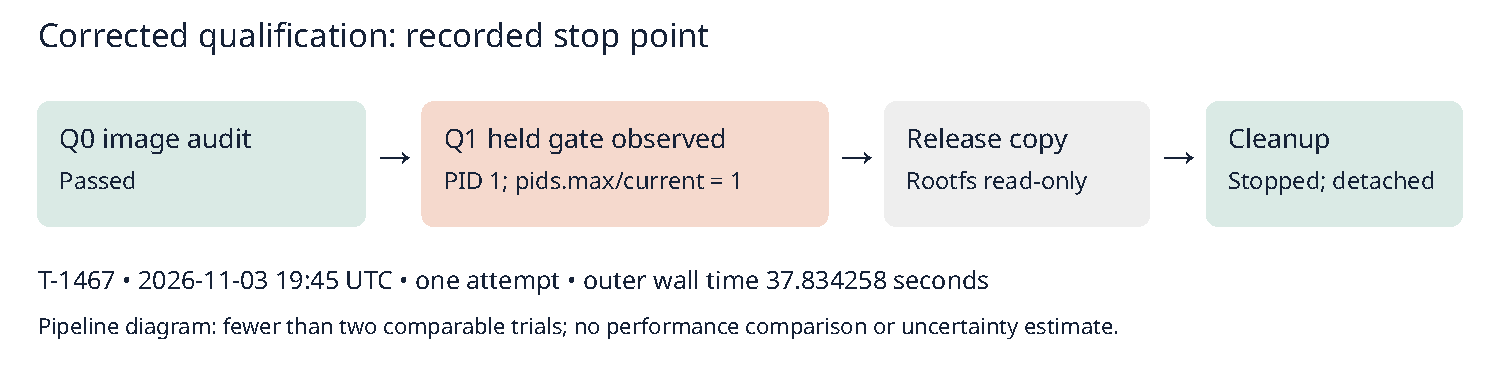
\includegraphics[width=\linewidth]{flow.pdf}

\begin{tabular}{lr}
Recorded quantity & Value\\\hline
Outer wall time (seconds)&37.834257627\\
Service CPU time (seconds)&8.649\\
Qualifier elapsed time (seconds)&5.554405689\\
Release-copy elapsed time (seconds, derived)&0.031484295\\
Completed qualification cases (count)&1 (Q0)\\
Conservative attempt debit (worker seconds)&600\\
Remaining allowance (worker seconds)&22800
\end{tabular}

\textbf{Evidence.} Parent-directory publication.json binds seven exact GitHub readbacks at commit be05306e7f before launch. Native receipts, image-file-inventory.json and extracted command/gate/ancestry records retain the observations. Release elapsed time is the command receipt's ended minus started monotonic time. Empty summary ancestry arrays reflect append-after-success ordering; granular records establish pre-release observations. The independent postreview accepts this distinction. There is one attempt, so the figure is a stop-point diagram, not a performance comparison.

\textbf{Limits and custody.} One 300-second, two-CPU, 2 GiB attempt reused the 4 GiB disk. Deadline remains 2026-11-04 06:00 UTC. All prior failures and debits remain; reservations total USD 58, actual dollars unmeasured. The worker records mounts and endpoint closed; captured observations show MainPID 0, absent cgroup and no associated loops. Bounded read-only debugfs extraction left disk metadata unchanged. The new worker disk digest is retained; the reviewer did not rehash it.

\textbf{Next source step.} Preserve the read-only root, one-process gate and tmpfs requirement. Review release publication through a verified directory descriptor into the existing container tmpfs, or a separately bounded owned tmpfs bind. Neither is a completed runtime correction. No scientific target was run.
\end{document}
